\chapitre{Marceline saute une coche, le vendredi 4 mai 1962 }{A onze ans, }{une fillette pourra être agacée par plusieurs choses. Par exemple, elle pourra détester se faire traiter de Bezo, comme tous les Belzile, ceux de Léonce, qui, en soixante ans, se sont succédé sur cette terre compliquée du 3e Rang Ouest de Saint-Fabien, une terre escarpée, constellée de roches, éloignée de tout, dont la richesse en cèdres et en érables avait été bûchée à quelques reprises. Si l’improbable surnom de Bezo était resté, fixé au vernaculaire comme synonyme de «colon plein de poux », celui de Belzile était disparu. Marceline, la dernière à pouvoir le porter au fin fond de ce rang jouxtant ceux de Saint-Mathieu, s’appelait Rioux depuis douze ans, à cause du grand Edmond, ce fier-à-bras de Saint-Simon qu’elle avait fini par marier. Les autres Belzile, ses jeunes frères et sœurs, étaient tous partis s’établir à Québec sous le nom de «Belzile \& frères, électricité plomberie», les garçons étant plombiers, les filles ayant épousé des électriciens.}

C’est ainsi que par défaut, l’aînée était l’héritière des espoirs trahis du grand-père Léonce, un brave homme plus enclin au rêve qu’à l’agriculture. En ce printemps de 1962, l’héritage n’était plus qu’une terre à bois laissée à elle-même, deux vieux bâtiments à moitié défoncés et une maison en bardeaux de cèdre qu’il faudrait retaper de fond en comble, la cabane des Bezo. Marie des Bezo détestait donc son statut social, ce qui ne l’aidait pas à entretenir des rapports amicaux avec les autres gamines à l’école du rang.

\begin{floatingfigure}[l]{40mm}
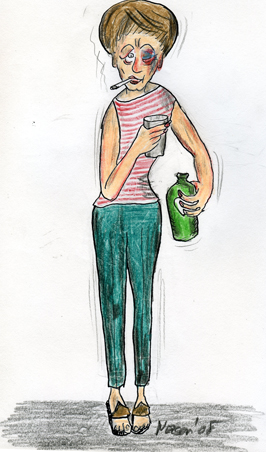
\includegraphics[height=60mm]{corps/chapitre10/img/personnage-marceline.jpg}
\end{floatingfigure}

En plus d’être ostracisée, puisque Bezo, une mouflette de onze ans pourra être exaspérée du fait d’être pointée du doigt comme étant la fille à Edmond, ce sombre bagarreur que tout le monde redoutait et dont on aimait raconter les exploits, le soir dans les chaumières, ou, pire, d’être la fille à Marceline, une assistée sociale maigre, probablement alcoolique, soupçonnée de mœurs légères que l’on apercevait occasionnellement, à l’hôtel, en compagnie des plus assoiffés noceurs du patelin. Avec sa vieille camionnette Fargo 1952, la «femme des Bezo» descendait régulièrement au village, mais parfois, elle faisait un crochet par l’hôtel. Ces jours-là, Marie devait se débrouiller seule pour le souper. Et quand sa mère revenait, avinée, bruyante et gauche, l’enfant faisait celle qui ne voulait pas l’entendre, qui ne voulait pas la voir, qui ne voulait pas l’embrasser, qui ne voulait surtout pas sentir son linge enfumé et son haleine de «fonds d’tonne». Certaines bonnes âmes avaient peine à endurer cette Bezo à la messe du dimanche accompagnée de sa petite fille. Pour ces gens, il aurait fallu qu’elle soit dénoncée en chaire et mise au ban de la communauté. Évidemment, si Edmond ne la maltraitait pas tant, colportait-on, peut-être boirait-elle moins. Mais, bon ! Heureusement que le grand tocson ne se pointait pas plus souvent le bout du nez. Marie Rioux avait donc honte de ses parents et apprenait à vivre sans avoir à ne parler à personne, en ne se préoccupant que d’elle-même, au point de se cacher de la nourriture pour être bien certaine de ne pas en manquer.

Passe encore être une paria, mais une Bezo de onze ans pourra particulièrement détester que l’on s’en prenne à son apparence. À onze ans, une gamine a de ces fiertés qui commencent à lui titiller les hormones. Marie qui, paradoxalement, marchait en tout temps la tête haute, n’hésitait jamais à regarder les gens dans les yeux, cela sans jamais sourire, et faisait constamment des miracles pour que ses vêtements aient l’air propres et neufs, abominait les visites de son père. C’est qu’en ces occasions, il lui arrivait de se ramasser quelques bonnes torgnoles qui lui déformaient parfois le visage pendant un jour ou deux. Comme résultat, les autres écoliers se moquaient plus que jamais, ce qui, chez elle, se transformait en rancœur et morgue. Heureusement, elle ne pouvait comparer sa situation avec celle de Marceline dont les traces de raclées nécessitaient souvent plusieurs semaines avant de se résorber complètement. Convaincue de ne pas mériter d’être maltraitée avec autant de méchanceté, elle s’interrogeait cependant sur sa mère au comportement général plus qu’erratique. L’ivresse n’expliquant pas toujours tout, il se pouvait que la Bezo ait poussé son Edmond à bout pour qu’il s’emportât ainsi, qu’il se mit à tout casser et à frapper ses proches. Il paraîtrait que depuis Ève et le serpent, la femme est souvent la cause de bien des débordements masculins. Donc, quand la petite saignait du nez, qu’elle avait la lèvre fendue ou la joue enflée, il se pouvait que ce soit par la faute de sa mère.

Edmond Rioux, brute dangereuse qui voyageait un peu partout au Québec pour des négociants de Montréal sévissant dans la voiture d’occasion, venait le plus rarement possible à Saint-Fabien. Et lorsqu’il se pointait, c’était la plupart du temps un vendredi en fin de soirée avec une «caisse de 24» et un «40 onces» de Bols ou de De Kuyper, ainsi qu’avec quelques billets de 20 \$ qu’il exigeait, telle une cérémoniale préivresse, qu’on lui sortît de sa poche de pantalon. Au printemps, Marie s’était retrouvée la lèvre ensanglantée pour s’être refusée à ce petit jeu. Le fier-à-bras s’installait dans la cuisine et se mettait à monologuer à voix forte sur sa vie de héros, sur ses bagarres les plus récentes, sur ses dernières trouvailles automobiles, sur ses patrons qui étaient de plus en plus voleurs et baise-la-piastre, sur René Lévesque qui avec son histoire de «nationalizâtion» de l’électricité, ”un autre mot à queue, bonyeu !”, s’était fait «r’placer les cordes vocales», ou encore sur les Canadiens qui ne savaient plus jouer au hockey tandis que les «Maple Leafs, ceuzes-là, y gâgnaient». À tout coup, il continuait son emportement sur le fait que l’eau du 3e Rang était «soufrée», qu’elle sentait les oeufs pourris, que si on «se lavait avec, on puait la charogne» et qu’elle n’était pas buvable. Ce stade franchi, il n’y avait qu’un échelon à gravir pour que sa cocotte pression n’explose. La plupart du temps, le prétexte était de nature sexuelle. Une pulsion bestiale intimait soudainement au colosse l’ordre d’exiger son dû et la Bezo devait dès lors obéir. Advenant que Marie soit dans les parages, elle était chassée avec force invectives. Puis, coincée contre le mur, Marceline subissait la virilité triomphante d’Edmond. Neuf fois sur dix, ces viols de fond de cuisine n’avaient pas de suite. Mais il arrivait qu’une grossesse s’ensuive. En ces occasions, la pauvre femme avait recours à la science d’Eugénie Jean, une bonne grand-mère catholique qui savait comment «empêcher la famille une fois le mal accompli». «Le Bon Dieu est bon, disait-elle, et Il peut pas être du bord des prêtres là-dedans !»

Dans ce monde sordide, Marie, petite fille sans jamais d’amis, s’était construite une planète à elle. Dans les fourrés autour de la maison, dans des clairières, près d’un des nombreux ruisseaux, à côté de «la grosse roche proche de la coulée», sous sa grande épinette à elle, voire sous la galerie d’en avant, elle entretenait des pièces imaginaires. Ici sa chambre de princesse d’où un beau chevalier viendrait un jour la délivrer. Là, le siège de son gouvernement. Plus loin, son salon de thé. À côté, son chalet de chasse. Puis le donjon de son château, le garde-manger de ses cuisines, son magasin de livres, sa petite chapelle du Bon Jésus et la scène d’où elle donnait ses concerts d’harmonica.

Un de ces sinistres vendredis, la gamine était alors âgée de neuf ans, son père lui avait offert une musique à bouche en lui révélant, à grand renfort de rires gras, tout ce qu’il y avait à dire :

- Tu tires p’is tu pousses, comme pôpa dans môman, p’is les notes vont jouer. Pratique-toé comme y faut, parce que quand j’vas r’venir, va falloir que tu m’jouses le «reel du mocking bird» !

Intriguée, stimulée, Marie était disparue. Dès l’aube du samedi, elle s’était aménagé une salle de concert sur une hauteur à quelques arpents de la maison et s’était mise à apprivoiser l’instrument. Il lui avait fallu une journée pour pousser «Frère Jacques», deux jours pour interpréter «Le cowboy fait le tour de la montagne» et un mois pour crachoter l’«Oiseau moqueur». Bien sûr, ses notes étaient approximatives, pleines de parasites mal discriminés, les demi-tons étaient escamotés, mais l’essentiel y était. On pouvait reconnaître les pièces qu’elle livrait. Elle eut besoin de moins d’un an pour savoir tirer le maximum de son «ruine-babines», en compensant pour certaines «notes noires» impossibles à rendre. Elle apprit à jouer tous les cantiques qu’elle connaissait, toutes les chansons qu’elle entendait à la radio, ou, quand le signal du Pic Champlain entrait assez fort dans les oreilles de lapin, à la télévision, une vieille Sylvania qui, une fois sur deux, nécessitait qu’on lui administrât un violent choc sur le côté pour fonctionner.

En partant de chez elle, Marie devait marcher près de trois kilomètres pour parvenir à l’école élémentaire, la «‘tite école» située au deuxième rang. Quand il faisait beau, le voyage était agréable et c’est en chantonnant ou en jouant de son harmonica qu’elle montait et descendait les innombrables côtes. Elle s’arrangeait cependant pour se mettre en route bien avant l’heure, question de ne rencontrer personne en chemin. Surtout les trois frères Jean-Pierre, Jean-Paul et Jean-Marc Roy. Elle les détestait tellement, eux et leur puanteur de souillon, qu’elle leur avait consacré une cérémonie. S’arrêtant devant une grosse roche à quelque 200 mètres de sa maison, elle la frappait à grands coups de trique, une «p’tite hart» comme elle le disait, à défaut de pouvoir le faire sur les garnements. C’était particulièrement vrai les jours où le plus vieux, Jean-Pierre, s’était appliqué à se faire rouler le farcin encroûtant ses bras, avec le pouce de la main opposée.

Mais s’il pleuvait ou crachotait ou poudrait, le trajet pouvait être un supplice. Elle arrivait parfois transie et Rhéa Théberge, l’institutrice, devait alors l’installer près du poêle. L’hiver, en période de grand froid, sa mère l’ayant autorisée à dormir à l’école, c’était la délectation suprême : elle s’amusait sur l’harmonium de la petite pièce qui servait d’étude à la résidente. C’est que flairant un talent certain, la jeune femme avait commencé à initier Marie à la logique musicale grâce à ce vieil instrument à vent. Encore là, Marie apprit tellement vite qu’à onze ans, elle pouvait jouer sans fausse note et avec les bons accords, une dizaine de cantiques, dont «J’engageai ma promesse au baptême», «Regarde avec amour», «Dans cette étable» et «Nouvelle agréable».

Entre elle et la demoiselle Théberge, une sorte d’entente s’était tissée. Comprenant que Marie, une enfant brillante pleine de potentiel, était molestée et laissée à elle-même, elle la prit sous sa houppe. Et plus encore. Elle la mit au fait des plaisirs de la connaissance, lui prêta des livres, des recueils et des revues. Elle l’initia au dessin, lui enseigna comment ménager ses crayons de couleur. Elle lui apprit à écrire de la musique. Elle en fit son adjointe pour assister les plus jeunes, de petits malheureux qui eurent ainsi à subir le caractère autoritaire, sec et contrôlant de la gamine. Il lui arriva même de la garder avec elle le soir, quand il faisait beau, surtout vers les fins de mois alors que chez les Bezo, il n’y avait plus grand-chose à manger. Le subterfuge pour que Marceline accepte était de dire qu’elle avait besoin de Marie, «une petite si raisonnable», pour l’aider à faire le ménage ou à rentrer du bois ou à corriger des cahiers, ce qui était parfaitement faux. Ces soirées n’étaient que prétextes à musique, l’harmonium étant poussé au maximum de son potentiel. Qui dort dîne.

Un jour, voyant la petite fille souffrir des quolibets que des enfants, dont les frères Roy, lui administraient en raison de son œil amoché, Rhéa se choqua et admonesta les galopins de sérieuse manière. Sur l’heure du midi, alors que les élèves étaient tous dehors en train de jouer, sauf peut-être les rares chanceux qui n’habitaient pas trop loin de l’école, elle essaya de faire parler Marie. Mais pas une seule parole ne put sortir tellement la boule qui lui bloquait le pharynx était énorme. Elle la prit alors dans ses bras. Après un réflexe de recul, la petite laissa la chaude affection de Mlle Théberge l’enrober et, malgré d’héroïques efforts, éclata en sanglots. Ce que voyant, l’institutrice en fit autant. S’il n’est pas exagéré de dire que toutes deux en gardèrent toujours un souvenir précis, il est surtout important de constater que, dans l’immédiat, les liens les unissant s’en retrouvèrent renforcés. Marie fit de Rhéa sa source unique de tendresse, de compréhension et de savoir. Tant pis pour Marceline qui n’osait s’adonner à de telles effusions.
S’il est vrai que chaque humain est censé connaître un «vendredi noir» au moins une fois dans le courant de sa vie, celui de Marie survint le 4 mai 1962.

Verre de gin dans une main, cigarette dans l’autre, Edmond semble de bonne humeur, assis, jambe croisée, sur le côté de la table de cuisine. Il s’est pointé, une heure plus tôt, au volant d’une Chevrolet Impala SS flambant neuve, une 350, avec sièges baquets, hard-top, carrosserie rouge et garnitures blanches. Apercevant la fillette, il lui demande de lui interpréter le «Mocking Bird» avec son harmonica. Mais comme il est particulièrement ivre et désagréable, elle refuse.

- J’t’ai dit de jouer, bonyeu !

- Laisse-moi tranquille, pleurniche-t-elle en manœuvrant pour s’échapper.

Malgré sa balourdise, il l’attrape par son tablier couvre-tout et la tire sur lui.

- Fais-y pas mal, supplie Marceline, pointant de son verre de gin.

- Toé, ta yeule !

En tentant de se libérer, Marie se met à crier, presque hystérique.

- Lâche-moi, lâche-moi, lâche-moi !

- Ah c’est comme ça que tu me remercies ?

D’une main, il la saisit par les cheveux et de l’autre, il lui fouille les poches de son couvre-tout. Comme il l’espérait, il découvre l’harmonica et, sourire en coin, la pose par terre entre ses deux souliers.

- Qu’in !

À coups répétés de talon, il écrase l’instrument qui se retrouve en débris à tout jamais perdus. Marie est épouvantée et ses hurlements atteignent l’insupportable.

- T’es méchant, méchant, méchant !

Pour toute réponse, Edmond lui allonge la gifle du siècle, ce qui propulse la gamine, la tête donnant violemment contre le mur de petites lattes.

- Décâlisse, j’veux pu te voir la face icitte !

Plus morte que vive, Marie s’en va alors se réfugier dans sa chambre, à l’étage. Même si elle sent son visage enfler, son cœur grossir, sa haine décupler, elle se couche et tente de convaincre ses grands yeux sombres de se fermer, d’oublier l’image de sa musique à bouche aplatie et en mille miettes.

En bas, le temps file. Edmond en est rendu à l’étape libidineuse et pour la énième fois, Marceline doit subir ses molestations. Pourtant, cette fois, il y a variante. L’ivresse pesant de tout son poids, la brute a fort à faire pour se placer en situation d’assouvir sa fureur bestiale. Même qu’il doit se reprendre et s’aider de la main, pour finalement renoncer, ce qui a l’heur de le mettre vraiment hors de lui.

- Bonyeu d’bonyeu, t’es aussi bandante qu’une couenne de lard !

La malheureuse se retrouve arrachée du mur où elle était aplatie, soulevée dans les airs et projetée vers la table qu’elle heurte du côté. Peut-être se fracture-t-elle quelques côtes, mais elle n’en parlera jamais. De toute façon, le pire est à venir. En titubant, Edmond s’approche, la relève violemment, l’adosse à la table pour qu’elle se maintienne à la verticale et lui décoche un direct sur l’œil. Heureusement, son ivresse ralentit le mouvement et Marceline a le temps de se protéger légèrement de la main. Reste que le coup atteint son but et que dans les heures qui vont suivre, l’œil gauche va se fermer dans un concert de tissus enflés et multicolores.

- C’est à ton tour, maman Bezo, se dit Marie réveillée par le vacarme.

Tout près de sa chambre, une grille circulaire en fer forgé donne sur le plafond de la cuisine près de la porte menant au passage. Vis-à-vis, sur le plancher, un dispositif semblable reçoit directement la chaleur de la fournaise de la cave. L’hiver, quand Marceline la chauffe sérieusement, Marie en profite toujours pour aller s’immobiliser sur l’un ou l’autre de ces grillages. Elle aime la sensation de l’air chaud montant sur ses jambes et elle affectionne de voir s’élever ses rebords de robe. En revanche, elle abhorre devoir descendre alimenter la chaudière. Phobie, superstition ou crainte naturelle ? Elle a peur des araignées qui, croit-elle, vivent en colonies dans les cordes de bois.

Dans la cuisine, Edmond est maintenant seul. Marceline s’est enfuie et le colosse ne dérage pas.

- Tu vaux pas de la marde, lui crie-t-il à tout hasard. Si ça continue, c’est la p’tite que je vas passer, bonyeu !

Puis, alourdie par autant d’alcool, la tête lui choit lentement, par petites secousses saccadées, jusqu’à ce qu’elle repose de profil sur la table. La main tenant sa cigarette s’affaisse, ce qui laisse tomber le mégot sur le prélart. N’entendant plus rien, Marie se met en frais de se convaincre de s’endormir, ce à quoi elle parvient au bout de quelques minutes.

Peu après, Marceline apparaît à la porte de la cuisine, un tisonnier de fer à la main, un fort bel objet à la poignée toute stylisée dont le grand-père Léonce avait hérité de son propre père. Doucement, elle s’approche, aperçoit la cigarette qui vient de finir de se consumer et écrase du pied les inoffensives cendres. Puis elle regarde son époux légitime, le malheur de sa vie, ce consommé de violence, ce violeur en série, cet être abject qui vient de menacer de s’en prendre à Marie et, lentement, comme si la fatalité avait inscrit ce geste dans le grand journal de sa vie, elle lève son pique-feu à bout de bras. Serrant les lèvres, tendant tous ses muscles, commandant toutes ses forces afin que son coup soit sans appel, elle l’abat de ses deux mains sur la tête de l’ivrogne. Étrangement, le bruit de cette mise à mort est peu dérangeant. C’est un bruit sourd, un peu semblable à celui du marteau qui défonce un crâne de veau. De la cavité ainsi créée, le sang se met à couler en abondance devant les yeux horrifiés de Marceline.

Sans trop calculer, elle tente de colmater la fuite avec un linge à vaisselle, mais rapidement, elle doit le remplacer par du plus costaud, un drap qu’elle se dépêche d’arracher à son lit situé dans la pièce voisine. Et là, malgré l’adrénaline qui lui fait bouillonner les plaquettes, elle va prendre le temps de réfléchir, les deux mains sur le drap placé en tapon sur la blessure. Le monstre doit être mort, pense-t-elle. Personne ne peut survivre à un impact d’une telle violence. Un plan ! Il lui faut maintenant un plan. Il lui faut se débarrasser d’Edmond avant que Marie ne se lève. Il faudra tout nettoyer, éliminer toutes traces du passage de la brute. Le traîner dehors, faire un grand trou, le pousser dedans, le rachever à coup de pelle au cas où il ne serait pas parfaitement trépassé, l’enterrer. Mais comment pourrait-elle vivre dans cette maison à côté des restes de son bourreau ? Et si elle vend et que des gens finissent par déterrer le squelette ? Non, il lui faut l’ensevelir ailleurs. Et son Impala ? Comment la faire disparaître ? La cacher dans le bois ? Et s’il y a enquête ? L’incendier ? Et la carcasse ? L’enterrer ? S’ils fouillent pour le corps, ils vont possiblement exhumer ce qui subsiste de l’auto. Le mieux n’est-il pas de tout déplacer le plus loin possible, le mort et sa bagnole? Mais où ? Pas au village, ni à Rimouski ! Quand on le découvrira, on saura qu’il est venu dans le coin et on la soupçonnera, elle, sa victime. Les victimes font toujours d’excellents coupables. Il faut plutôt ramener ce démon sorti de l’enfer d’où il est parti. En relâchant le drap, la jeune femme sait maintenant qu’elle a un vrai plan.

Elle ne trouve pas les clés de l’Impala, ni dans les poches du veston qu’Edmond a accroché sur le dos de sa chaise, ni dans celles de son pantalon où elle dégote cependant une liasse de 235 \$. Une fortune ! « T’aimes ça de faire fouiller d’in poches, mon Edmond !» Le fichu trousseau n’est ni sur la table, ni par terre. Malgré la douleur vive qu’elle ressent aux côtes, elle se précipite dehors, ouvre la portière du bolide et constate que les clés ont été laissées sur le contact. Sans hésiter, elle démarre et manœuvre la voiture de façon à ce que le pare-chocs arrière vienne frapper la deuxième marche de l’escalier menant à la grande galerie d’en avant. Comme si un incendie faisait rage, elle revient à la cuisine et enserre le cadavre par les aisselles pour le faire choir jusqu’à terre. Évidemment, le tissu imbibé de sang se défait de la plaie et un flot noirâtre commence à se répandre tout doucement sur le prélart. Marceline accourt à son lit, y arrache le deuxième drap et en entoure minutieusement la tête d’Edmond. Puis, forçant comme il ne lui était jamais arrivé de le faire, elle entreprend de tirer la lourde carcasse par les pieds. Elle ahane ainsi jusqu’à l’entrée, puis jusqu’à la galerie. Là, à genoux, elle place le fardeau sur le long, parallèle aux marches et, fermement, des deux mains, le pousse et le fait rouler jusqu’en bas.

Presque en panique, quasiment pétrifiée par la peur, elle tente de le glisser dans la malle. Mais elle n’y arrive qu’en partie, une jambe s’est bêtement coincée entre la marche et le pare-chocs. Et on jurerait que plus elle la secoue pour la dégager, pire c’est. Un instant, elle se voit devenir folle. Mais elle se ressaisit et coure prendre le volant. Hélas, dans son affolement, elle lance l’Impala à reculons, ce qui écrase le membre contre le bois vermoulu de l’escalier. Crouc ! Comment fait-elle pour contenir son besoin de hurler ? Elle l’ignore ! Sans perdre une seconde, elle embraie vers l’avant en aplatissant l’accélérateur, suivi, une seconde plus tard, du frein. Le véhicule bondit et s’étouffe. Si la jambe s’est dégagée, le tissu du pantalon est maintenant incrusté dans la chair et les os en une sorte de bouillie sanguinolente. Complètement révulsée, Marceline doit se reprendre trois fois avant d’arriver à se saisir de la patte rebelle pour la placer dans la malle. Et là, prise de nausée, elle a tout juste le temps de se pencher sous la galerie, une des pièces imaginaires de Marie. Après une courte pause de respiration, elle se précipite à l’intérieur vers son tas de linge sale. Deux draps vont lui servir à enrober de façon plus étanche le crâne défoncé et une taie d’oreiller, la jambe mutilée. Enfin, elle referme violemment le cercueil motorisé et grimpe à nouveau l’escalier.

C’est le bruit du moteur qui a réveillé Marie. Incitée à la prudence extrême par la douleur lancinante qu’elle ressent au visage, elle s’est levée et a regardé par sa fenêtre qui donne sur l’avant de la maison. Le toit de la galerie étant dans son champ de vision, elle a quand même pu constater, malgré la noirceur, que la voiture rouge avait été reculée jusqu’à l’entrée. Inquiète, elle a alors prêté l’oreille et a d’abord identifié le va-et-vient pressé de sa mère. Puis une sorte de glissement dont elle n’arrivait pas à déterminer l’origine. Pourquoi n’entendait-elle point son père gueuler comme d’habitude ? Et quelle était la nature de ces soupirs que l’on poussait comme si on se livrait à de sérieux efforts ? Elle s’est donc approchée de la grande grille de chauffage et a essayé de voir. C’est ainsi qu’elle a aperçu les mains de Marceline qui disparaissaient de son angle d’observation, des mains qui tiraient sur les pieds d’un corps dont la tête était enveloppée, un corps qui était celui d’Edmond.

Marceline marche sans arrêt entre l’évier et la cuisinière, sans savoir où elle se trouve. Elle rumine. Des images terribles défilent dans son ciboulot à une vitesse folle. Pour tenter de se calmer, elle se sert un grand verre d’eau, puis va à la salle de bain où elle essaie de se nettoyer les blessures qui la défigurent. Découragée, elle se brosse sommairement les cheveux et grimpe à l’étage.

- Marie, réveille-toi. On s’en va à Québec. Envoye, dépêche.

Faisant mine de rien, la petite fille se lève et s’habille. Dans la cuisine, Marceline lui tend un verre de lait qu’elle refuse de la tête.

- Viens-t-en, y est déjà cinq heures, faut décoller.

Pendant les trois heures du trajet, la périlleuse 10 jusqu’à Rivière-du-Loup et la dangereuse 2 jusqu’à Québec, pas un mot ne sera échangé à l’exception de :

- J’vas arrêter le char icitte sur le bord du chemin; va faire ton pipi.

Dès Kamouraska, l‘indicateur du niveau d’essence commence à l’inquiéter et son soulagement ne surviendra qu’à Sainte-Anne-de-la-Pocatière où un garage Texaco sera tout juste en train d’ouvrir. Le pompiste se souviendra probablement longtemps de sa première cliente de la journée, une femme au visage tuméfié, un œil complètement fermé, qui vint faire le plein avec une Impala SS 350 de l’année.

\begin{floatingfigure}[l]{60mm}
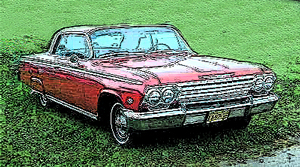
\includegraphics[height=30mm]{corps/chapitre10/img/voiture.jpg}
\end{floatingfigure}

Arrivée dans le bas de la ville de Québec vers 8 heures 30, Marceline gare la rutilante voiture sur la rue Saint-Joseph, presque au coin de la Couronne, à deux pas de l’Hôtel Saint-Roch. Elle s’empare du trousseau de clés, d’où elle retire celle de la malle arrière, et le remet sur le contact. Son plan est simple : ceux qui voleront l’auto éprouveront beaucoup de difficultés à mettre au jour le sépulcre d’Edmond. Ils prendront leur temps, soucieux de ne pas endommager une si belle automobile; il leur faudra bricoler et, au terme, quand le coffre finira par s’ouvrir, ils auront un cadavre sur les bras. Pendant ce temps-là, elle et Marie seront loin.

Avant de quitter, elle essuie d’un mouchoir tout ce qu’elle croit avoir pu toucher, elle abaisse les deux grandes fenêtres latérales de l’Impala et se met à marcher, Marie à sa suite, en direction du poste de taxis tout près de l’hôtel.

Assis dans sa Plymouth noire en train de lire l’Événement-Journal, un chauffeur les remarque et, du regard, interroge Marceline.

- Sur l’aut’ bord du pont de Québec, y a un restaurant avec plein de gars de truck. C’est là qu’on s’en va. Pis j’ai d’l’argent pour payer, ajoute-t-elle aussitôt en brandissant une partie de sa fortune.

Sans dire un mot, l’homme, habitué à d’aussi pathétiques cas de misère humaine, le quartier Saint-Roch étant ce qu’il est, accepte la course et les passagères s’installent sur la banquette arrière. Tout au long du trajet, la discrétion étant sa devise, il va se faire un devoir de ne pas les regarder par le rétroviseur.

- Ici ça fait-y, demande-t-il une fois le pont traversé. Le parking est plein de trucks et de vans.

- C’est b’en correct.

Yvette Carrier, serveuse responsable du comptoir dont les tabourets semblent plaire à certains clients, remarque, par une des grandes fenêtres latérales de l’établissement, un taxi de Québec duquel descend une adulte qui boite en se tenant les côtes d’une main et serrant celle d’une petite fille aussi amochée qu’elle de l’autre. Du coin de l’œil elle les regarde entrer et venir s’asseoir juste en avant d’elle. Comme elle a probablement tout vu ce qui était possible de voir, elle ne fait mine de rien et se tourne à nouveau vers la grande baie vitrée pour fumer sa cigarette.

- Ça va être quoi, les madames, demande-t-elle finalement, son carnet de factures à la main.

- On a faim, répond Marceline. On voudrait des œufs avec du bacon pis des toasts.

- Comment les œufs ?

- Virés de bord. Pis du café pour moi et du lait pour la p’tite.

Dix minutes après avoir été servies, ni l’une ni l’autre n’ont avalé quoi que ce soit. C’est à peine si la jeune femme a trempé ses lèvres dans le café.

- Sont pas bons, mes œufs ? questionne Yvette Carrier.

Marceline repousse son assiette en regardant Marie.

- C’est pas qui sont pas bons, c’est qu’ils passent pas.

- Ouin, ça pas d’l’air de filer pantoute, à matin ?

- Mettons que ç’a déjà été mieux.

- J’vois b’en ça !

- On s’en va dans ma famille à Rimouski, ment-elle.

Puis, après quelques secondes de silence.

- Il a pas mal dépassé les bornes cette nuit.

La serveuse tire sur sa cigarette d’un air entendu.

- Pauvre ‘tite madame, voir si ç’a du bon sens ! Pis c’te p’tite fille-là aussi. Y en a-t-y des chiens sales !

Le plan de Marceline semble se dérouler tel que prévu.

- Vous connaîtriez pas quelqu’un, des fois, ici dans votre restaurant, qui serait prêt à nous prendre jusqu’à Rimouski ?

Yvette Carrier la regarde un instant sans parler, puis lui fait un signe de patienter. Elle s’approche d’un quinquagénaire à casquette, un mal rasé en train d’avaler un déjeuner tardif, et amorce une brève discussion au cours de laquelle elle pointe à quelques reprises vers Marceline et Marie. Puis elle hoche de la tête et revient à son comptoir.

- Tony, là-bas, il va vous prendre. Il travaille pour Rimouski Transport et il fait la run Montréal – Gaspé. Il va vous laisser en passant. C’est un bon gars, même s’il est pas beau.

Comme son interlocutrice semble hésiter, elle ajoute :

- Vous avez pas besoin d’avoir peur.

Quinze minutes plus tard, Marie se retrouvait assise entre ledit Tony, grand sec à l’éternelle cigarette, et sa mère, une serviette de table mouillée tenue sur l’œil, dans la cabine d’un camion de livraison avec comme destination, le Bas-du-Fleuve. À quelques reprises, à voix à peine audible, le chauffeur va tenter d’amorcer une conversation, aussi bien avant qu’après la halte rituelle au Martinet de La Pocatière. Mais Marceline ne mordra pas et Marie sera muette comme une carpe dépressive. Cependant, à la hauteur du Bic, il ne pourra plus se contenir.

- Ce n’est pas de mes affaires, madame, mais Yvette m’a dit que la p’tite avait rien mangé et rien bu au comptoir. P’is tantôt au Martinet, elle a rien voulu prendre. Même pas un verre d’eau. Elle parle pas, elle bouge pas. C’est pas normal pour un enfant de son âge. À vot’ place, j’irais voir un docteur. Elle a un problème, c’est sûr.

- Ouin, c’est ce que je vas faire en arrivant à Rimouski.

Mais elle ne le fera pas. Car une fois descendues de l’énorme «Inter», Marie et elle marcheront trois pâtés de maisons jusqu’à une boutique de fleuriste de la rue Saint-Germain.

- Lise, fait-elle à une petite bonne femme toute ronde, rose et rieuse, j’ai besoin de toi.

Apercevant sa cousine aussi mal amochée, Lise Laplante, la propriétaire, s’exclame à grand renfort de gestes.

- Il vous a encore battues, le verrat ?

- Y a rien de neuf là-dedans, lui rétorque Marceline. Écoute, j’ai besoin de toi.

- Que c’est que je peux faire ?

Elle lui explique devoir absolument s’en aller chez elle, à Saint-Fabien. Elle en a à peine pour deux heures, mais elle ne peut amener Marie. Si Lise avait la gentillesse de la garder et d’essayer de lui faire avaler quelque chose, elle lui en serait reconnaissante.

- Elle a rien mangé depuis hier. A va pas bien. Et si en plus, tu pouvais me prêter ton char, ça m’aiderait pas mal.
Habituée aux extravagances de sa parente, Lise ne dit mot, ouvre un tiroir et lui tend un trousseau de clés.

- Le char est en arrière du magasin. Mais pourquoi que tu veux t’en aller à Saint-Fab, là, maintenant ?

- C’est une affaire de rien, mais j’peux pas t’en parler. Fais-moi confiance, y a rien de méchant.

\begin{floatingfigure}[l]{30mm}
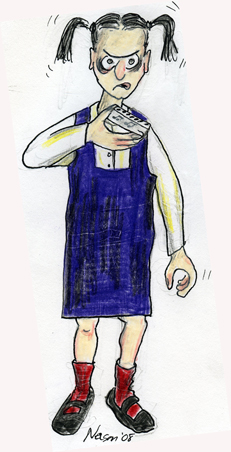
\includegraphics[height=50mm]{corps/chapitre10/img/personnage-marie-jeune.jpg}
\end{floatingfigure}

Une demi-heure plus tard, Marceline, la femme des Bezo, est chez elle en train de tout nettoyer «à grande eau». Il ne faut plus qu’il reste quoi que ce soit d’Edmond. Même pas l’air qu’il a respiré. Elle astique son prélart, lave verres et cendrier, brûle le linge à vaisselle, fait disparaître les traces de pneu qu’a laissées l’Impala en avant de la maison et les traces de sang laissées par la jambe, replace les bouteilles vides dans leur caisse, sans oublier le «40 onces» à moitié plein, place le tout sur la banquette de la voiture – elle les jettera dans les poubelles de sa cousine fleuriste - et fait le tour vingt fois. Ce faisant, son regard porte sur la grille d’air chaud et elle revoit sa gamine s’y amuser à l’observer et à lui parler au travers des orifices. Un doute vient l’habiter. Et si, hier soir, Marie avait été éveillée et avait vu toute la scène ? Ou une partie de la scène ? Elle ne dormait probablement pas, ce matin, quand elle lui a dit de sortir du lit; contrairement à son habitude, elle s’est levée immédiatement. Et si elle a vu quelque chose, elle est peut-être en état de choc, d’où la raison pourquoi elle ne mange pas, ne bois pas et ne parle pas. Et si elle débloque, qu’elle se met à raconter des choses ?

Inquiète, Marceline saute dans l’auto et revient à Rimouski le plus vite qu’elle le peut. Quand elle entre dans l’arrière-boutique de la fleuriste, elle constate que Marie est en train de grignoter une DairyMilk de Cadburry. L’ayant entendue arriver par l’arrière, la commerçante passe la tête sur le rebord du rideau qui agit comme porte entre la pièce et la boutique.

- Elle a d’l’air à filer mieux, explique la cousine Lise. Elle m’a dit qu’elle avait un peu faim. Fait que je lui ai donné d’la liqueur, un bon cream soda, et une bonne barre de chocolat. Hein ma chouette ?

Marie ne bronche pas.

- Ensuite, elle m’a conté qu’elle avait fait un beau voyage dans un camion avec un monsieur appelé Tony. C’est-tu vrai ça ?

Marceline hésite avant de répondre.

- Mettons qu’elle a une b’en grosse imagination. Surtout ces temps-citte !

- Ah ! Je sais c’est quoi ! J’en ai une du même âge à la maison. Ça en raconte, des histoires !

Ce soir-là, quand Lise les aura ramenées dans le 3e Ouest, toutes deux s’écraseront de fatigue. Marie aura peine à grimper jusqu’à sa chambre.

Le lendemain matin, pendant que Marceline est occupée à touiller sa soupane aux pommes et à la cassonade pour faire comme si de rien n’était, Marie descend, tout habillée, sa joue encore enflée. La mère, malgré ses pressentiments, tente de se faire le plus accueillante possible. Elle raconte être allée chercher les derniers fruits dans la cave pour préparer ce «bon gruau». Mais l’arôme du festin ne peut rien contre le visage dur, noir, mauvais de la fillette.

- J’en veux pas de ton gruau, je veux partir d’ici, Je veux plus être avec toi.

- Mais voyons, ma pitchounette.

- T’es méchante. Tu m’as pas défendue quand il m’a battue, tu l’as laissé faire quand il a détruit ma musique à bouche, ma belle musique à bouche, maudit ! Mais toi, par exemple, tu t’es défendue. Je t’ai vu le sortir. Pis après, tu m’as fait passer pour une menteuse chez matante Lise. J’veux p’us rester ici, j’veux m’en aller. T’es aussi méchante que lui ! P’is j’ai trop peur qu’il revienne !

Et l’enfant de déguerpir vers ses contrées imaginaires. Marceline ne la reverra que le soir et n’arrivera pas à lui parler. En fait, elle n’arrivera plus jamais à lui parler. Pire, personne, à l’exception de Rhéa Théberge, n’arrivera à le faire, et encore. Marie ne fera plus de devoirs, n’aidera plus en classe, ne touchera plus l’harmonium et écrira n’importe quoi sur ses feuilles d’examen de fin d’année.

Tant et si bien que le lundi 18 juin, début de la dernière semaine de classe, l’institutrice constate qu’elle va devoir recaler la petite, lui faire reprendre sa sixième année, elle qui en sait beaucoup plus que les grands de septième, tant la somme des points perdus depuis le début de mai est importante. Toutes ses tentatives d’en parler avec elle ont été inutiles, Marie s’étant refermée. Et malgré les pluies abondantes en cette fin de printemps, elle a préféré marcher les trois kilomètres matin et soir.

L’absurdité de la situation émeut Rhéa au point où sur la fin de l’après-midi, elle se pointe chez Marceline occupée à sarcler son jardin, un enclos cintré d’une ancienne clôture en pieux de cèdre désormais incapable d’arrêter les chevreuils. Marie n’étant visible nulle part, elle va droit au but. La petite est brillante, bourrée de talents, assoiffée d’apprendre. Pour tout dire, elle est de loin la meilleure élève qu’elle n’a jamais eue dans sa carrière. Mais il s’est passé quelque chose en début mai. Depuis, c’est la dégringolade. À pic !

- Saviez-vous, madame Rioux, que votre enfant joue de l’harmonium mieux que moi ?

Aucune réponse. L’enseignante constate que son interlocutrice semble davantage intéressée aux manœuvres d’une libellule. Mais elle poursuit.

- Saviez-vous qu’elle sait lire et écrire de la musique, clé de sol, clé de fa ? Qu’elle a lu, cette année, un livre par semaine, incluant tous les Marcel Pagnol que j’ai pu trouver ? À onze ans ? Qu’elle faisait faire leurs devoirs aux plus jeunes ?

- Ouin, elle m’en a parlé.

Marceline a de la difficulté à ne pas rougir devant un si grossier mensonge. Elle se ressaisit et ne donne pas à Rhéa Théberge le temps de poser une nouvelle question.

- Écoutez, mam’zelle Théberge, je sais que ma fille est pas pire, mais je vois pas où c’est que vous voulez en venir.

- À ceci !

L’enseignante ouvre brusquement sa mallette en cuir brun. Elle en extirpe quelques feuilles qui, explique-t-elle, démontrent que Marie n’a pas répondu aux questions des examens. Et, avec le passif accumulé depuis le début mai, elle ne peut être promue en septième, ce qui constitue une aberration majeure. À un point tel, qu’on ne peut se contenter de ne rien faire, ce qui suppose qu’il faut absolument la changer de milieu. Lui donner une chance d’assumer son potentiel. De toute façon, il faut se faire à l’idée qu’elle est à la veille de «changer d’air». Dès le secondaire, elle devra effectivement passer ses semaines en bas, au village, chez des parents, chez des amis ou dans une pension. Il lui sera devenu impossible de voyager matin et soir. Aussi bien devancer d’un an, non ?

Marceline commence à être agacée.

- Pourquoi vous me dites tout ça, là ?

- Parce que je veux vous aider à lui trouver une place quelque part en ville pour qu’elle fasse sa septième année. J’ai pas le droit, mais je suis prête à arranger ses notes pour qu’elle monte quand même.

- Où en ville ?

- À Rimouski, à Québec, à Montréal. Quelque part où elle sera prise en charge et où elle pourra faire des études à sa mesure. Madame, votre fille est brillante et, ici, dans les rangs de Saint-Fabien, elle est bloquée, fermée, en état de régression.

Rhéa Théberge lorgne le jardin comme si elle voulait inventorier les espèces qui y poussent.

- Et, si je l’ai bien comprise, elle a une peur bleue de son père …

- Son père, ça fait un siècle qu’on l’a pas vu, coupe la femme des Bezo.

- Elle doit partir, madame, c’est pour son bien.

- Écoutez donc, vous ! J’vous trouve b’en effrontée.

- Madame Rioux, j’aime beaucoup votre fille. Elle mérite qu’on s’en occupe, qu’on lui dégote une place quelque part.

Marceline tente de pénétrer l’intérieur des yeux de Rhéa.

- Elle va vraiment doubler son année ?

- Oui, ses notes sont terribles.

- Mon Dieu seigneur !

- Dites-moi juste que vous allez y penser.

Pour y penser, elle va y penser ! Et sans perdre de temps.

Deux jours plus tard, Marceline va débarquer chez sa cousine fleuriste à Rimouski et quand elle en repartira en fin de soirée, le sort de Marie aura été tracé. La fillette, dont l’imagination est très fertile au point qu’il faut s’en méfier, sera placée en pension chez «matante Lise» et le plus tôt sera le mieux. Durant l’été, elle rendra service dans la boutique. Par exemple, elle fera le ménage, elle apprendra à faire des bouquets, à livrer de petites commandes et même à recevoir les clients. Sans compter qu’elle pourra devenir amie avec Colette, la fille unique de Lise. Et, en septembre, elle ira faire sa septième année à l’école Saint-Pie-X, à deux pas de la maison des Laplante, ce qui ne l’empêchera pas de continuer à donner un coup de main au commerce de la rue Saint-Germain pour rembourser sa pitance. Ensuite, on verra !

Ce qui fut fait. En un an, il se passa quatre choses importantes dans la vie de Marie Rioux, plus jamais Bezo. Loin de sa mère, loin du 3e Ouest, repliée sur elle-même, elle se transforma, dès septembre, en première de classe un peu chipie et ne laissa jamais personne, même les jumelles Thibault, les filles du docteur, lui ravir sa place. Puis, en octobre, elle découvrit un violoncelle enfermé dans le placard du salon, un instrument dont se targuait de jouer, à l’occasion, ce bon diable de Lucien Laplante, le mari tout rondelet, jovial, inoffensif et soumis de Lise. Comme si cela allait de soi, elle se l’appropria et entreprit d’en tirer des sons avec l’aide complice de son propriétaire, une aide enjouée qu’elle toléra néanmoins avec distance et prudence, ainsi qu’avec les conseils occasionnels de Rhéa Théberge qui venait la visiter de temps à autre. Ensuite, en décembre, la fillette refusa énergiquement d’aller passer le congé des fêtes chez Marceline. Elle tint tête à tout le monde et vécut son premier Noël, pour peu que ses souvenirs soient fiables, sans grincements, sans pleurs, sans alcool et sans violence. Enfin, en mars, le conflit avec sa cousine Colette devint insoutenable. Le caractère de l’une étant mauvais, la jalousie de l’autre atteignant des sommets, les deux jeunes filles cessèrent à tout jamais de se parler. Tant et si bien qu’à la fin de l’année scolaire, il fut convenu de retourner Marie chez sa mère.

********************************

Il ne reste plus qu’un long paragraphe, presque toute une page calligraphiée, avant que la lettre de Marceline ne soit terminée. Ému, Timothée poursuit sa lecture, déchiffrant, sans humeur, le texte constellé de fautes et de tournures laborieuses. Tellement qu’il lui arrive de devoir reprendre des passages jusqu’à trois fois avant d’en saisir le sens.

- «Mais il y avait un homme qui vivait avec moi, récite-t-il au bénéfice de Romain qui fixe les motifs du tapis. Quand tu as vu ça, tu ne l’as pas accepté du tout. Tu n’as pas voulu rester avec moi une minute de plus. Tu avais très peur et tu m’en voulais encore. Autant que l’année précédente. Tu as crié. Tu as tout fait pour t’en aller. Ce qui fait que j’ai fini par te placer chez ma sœur Denise à Québec. En attendant, tu es allée coucher chez Mlle Théberge. Et comme je craignais que tu leur bavasses tout, je leur ai dit qu’au sujet de ton père, tu racontais des histoires tirées de ton imagination et qu’il ne fallait pas qu’elles te croient. Ça m’a fait beaucoup de peine, je t’aimais tellement. À partir de là, tu as continué de t’enfermer encore plus creux dans ton monde de musique où tu étais à l’abri de tous ceux qui pouvaient te faire mal.» Ouin, Maman et sa musique …

- Continue …

- « Quand ton père à brisé ta musique à bouche, c’était ton monde qu’il massacrait. Sur le coup, je ne l’ai pas compris et tu m’as haïe parce que je n’avais rien fait pour l’empêcher. Pourtant, tant que tu as été avec moi, j’ai toujours essayé de te protéger, mais il faut croire que je n’en ai pas été capable comme il aurait fallu, comme tu l’aurais voulu. Après, j’ai essayé de te parler, mais tu n’as jamais voulu. Ce qui fait que je me suis contentée d’avoir de tes nouvelles par Denise que j’ai appelée toutes les semaines. C’est comme ça que j’ai su que tu étais toujours la première de ta classe et que tu étais entrée au conservatoire où tu étais la meilleure. Mais ça, ce n’est plus mon histoire. Elle est finie mon histoire. J’ai déclaré que ton père avait disparu et la police ne l’a jamais retrouvé.»

Romain se désenrhume.

- Sacrament !

- Attends ! Ce n’est pas terminé. «Bonne chance, ma petite Marie, je t’ai toujours beaucoup aimée et je t’aimerai toujours. De ta maman Marceline Belzile qui te demande pardon pour ne pas avoir été capable. C’est à mon amie, madame Rose Joncas, que je vais donner cette lettre pour qu’elle te la donne.»